% For TeXworks
\makeatletter
\declare@file@substitution{revtex4-1.cls}{revtex4-2.cls}
\makeatother

% Define document class
\documentclass[twocolumn,twocolappendix,linenumbers]{aastex631}

% \usepackage{showyourwork}
\usepackage{amsmath}
\usepackage{amssymb}
\usepackage{graphicx}
% \usepackage{layouts}
\usepackage{xcolor}
% \usepackage{upgreek}
\let\tablenum\relax
\usepackage{siunitx}
\usepackage{xspace}

% user-defined commands
% \newcommand{\yes}{\textcolor{green}{\checkmark}\xspace}
% \newcommand{\meh}{\textcolor{black}{$\sim$}\xspace}
% \newcommand{\no}{\textcolor{red}{$\times$}\xspace}
\newcommand{\osuaffil}{Department of Astronomy, The Ohio State University, 140 W. 18th Ave, Columbus OH 43210, USA}
\newcommand{\ccappaffil}{Center for Cosmology and AstroParticle Physics, The Ohio State University, 191 W. Woodruff Ave., Columbus OH 43210, USA}
\newcommand{\aFe}{[$\alpha$/Fe]\xspace}
\newcommand{\vice}{{\tt VICE}\xspace}
% \newcommand{\hydro}{{\tt h277}\xspace}
\newcommand{\todo}[1]{{\color{red}#1}}

% Citation aliases
\defcitealias{johnson_stellar_2021}{J21}
\defcitealias{leung_variational_2023}{L23}
\defcitealias{dubay_galactic_2024}{D24}

\shorttitle{Two-Infall in VICE}
\shortauthors{Dubay et al.}
% \linespread{1.8}

\begin{document}

% Title
\title{A Two-Infall Star Formation History with Outflows and Radial Migration}

% Author list
\author[0000-0003-3781-0747]{Liam O.\ Dubay}
\affiliation{\osuaffil}
\affiliation{\ccappaffil}
\author[0000-0001-7258-1834]{Jennifer A.\ Johnson}
\affiliation{\osuaffil}
\affiliation{\ccappaffil}
\author[0000-0002-6534-8783]{James W.\ Johnson}
\affiliation{Observatories of the Carnegie Institution for Science, 813 Santa Barbara St., Pasadena CA 91101, USA}
\affiliation{\osuaffil}
\affiliation{\ccappaffil}
% \author[0000-0001-7775-7261]{David H. Weinberg}
\author{coauthors}

\correspondingauthor{Liam O.\ Dubay}
\email{dubay.11@osu.edu}

\begin{abstract}
    Abstract.
\end{abstract}

\section{Outline}

\subsection{Outline of Key Plots}

\begin{itemize}
    \item The turn-over in [O/Fe] evolution due to the second infall epoch produces a peak in the stellar distribution at intermediate [O/Fe], which is not observed in APOGEE.
    \item Attempts to fix the problem with the [O/Fe] distribution in the thin disk end up creating issues with other observables, such as the thick/thin disk surface density ratio, the SN Ia DTD, or the age-metallicity relation.
    \item The equilibrium model, if accurate, places very strict limits on the two-infall model, moreso than for other models.
    \item A short ($\sim200$ Myr) star formation hiatus early in the history of the disk is sufficient to produce a bimodal distribution of [O/Fe] without altering the gas infall prescription. This is distinct from the star formation hiatus produced by the two-infall model.
\end{itemize}

\section{Introduction}

% To add: Karma Gallart (2019) three-infall-ish, Kobayashi metallicity limit for SNe Ia and sub-Chandra

The two-infall model has long been proposed to explain the formation of the Milky Way's thick and thin disks. The infall history of any given region of the disk is described by two successive, exponentially declining bursts, whose timescale may vary as a function of radius. The first infall, which forms the thick disk, has a short timescale, typically on the order of $\sim1$ Gyr. The second infall forms the thin disk and has a much longer timescale, typically $\sim4-10$ Gyr.

\subsection{Summary of Two-Infall Papers}

% Summary of two-infall papers
\citet{matteucci_galactic_1989} modeled the galaxy with a two-component model, a one-zone model for the halo and concentric shell zones for the disk. They used a simple exponential gas infall (so not yet a two-infall model), where the infall timescale increased proportionally with radius. They studied cases with primordial and pre-enriched gas infall, finding that the former produces a more realistic metallicity distribution in the Solar neighborhood. Their inside-out disk evolution produced good agreement with observed abundance gradients.

\citet{chiappini_chemical_1997} presented the first two-infall model of the MW disk. They adopted an inside-out prescription for the formation of the thin disk, with the timescale of the second infall increasing linearly with radius. They assume the formation timescale of the thick disk is 1 Gyr, and the time of the second infall is 2 Gyr. They also assume a lower threshold on the gas density required for star formation, which produces a star formation hiatus at the end of the thick disk phase. They also noted the ``loop'' that appears in the \aFe--[Fe/H] relation during the thin disk phase. They mostly compare to Solar neighborhood data.

\citet{chiappini_abundance_2001} updated their model to fit the observed abundance, stellar, and gas gradients in the Milky Way disk. They find that a density threshold for star formation, making a gap in star formation between the halo and disk phases, is necessary to reproduce observational data. They argue that the details of halo formation also have a strong impact on the outer disk. No radial flows or outflows. I'm confused about their distinction between halo and thick disk, if any.

\citet{chiappini_oxygen_2003} compare model predictions of C, N, and O to Milky Way and other spiral galaxy data. They predict a very slow enrichment between the birth of the Sun and present day, which they claim is due to their adopted gas density threshold for star formation (the infall rate is low enough that the SFR oscillates from timestep to timestep).

\citet{matteucci_effect_2009} investigated different SN Ia delay time distributions using the \citep{chiappini_chemical_1997,chiappini_abundance_2001} model. They use a model for the full disk but compare only to Solar neighborhood data. They concluded that some prompt SN Ia enrichment is necessary to match observed abundance patterns.

\citet{spitoni_effects_2009} relaxed the instantaneous recycling approximation in two different ways: galactic fountains (i.e., SN ejecta are launched out of the disk and take some time to return) and metal cooling (i.e., newly-enriched hot gas takes time to cool before it can form stars). They found that fountains do not strongly affect the evolution of the $\alpha$-elements for short (few hundred Myr) timescales. The effect of a metal cooling timescale is similarly negligible if the yields are not dependent on metallicity.

\citet{spitoni_effects_2011} find that a two-infall model of the disk without gas exchange produces a radial metallicity gradient which is too shallow. They implement an inward radial gas flow on the order of $\sim0-4$ km s$^{-1}$ which varies with radius, and find that it improves agreement with the observed gradient. However, they found that a variable star formation efficiency with radius in combination with a gas density threshold for star formation could also reproduce the observed gradient without radial flows.

\citet{spitoni_effect_2015} add a simple radial migration scheme to the model of \citet{spitoni_effects_2011}. They adopt stellar velocities of $\sim 1$ km s$^{-1}$ and assume that some fixed fraction of stars born at a given radius will end up in the Solar vicinity (10\% of those born at 4 kpc and 20\% at 6 kpc). This mimics the results of previous dynamical models such as \citet{minchev_chemodynamical_2013}. They find that by including stellar migration, they are better able to reproduce the high-metallicity tail of the local metallicity distribution, and they also argue that they constrain the migration speed to $0.5 < v < 2$ km s$^{-1}$ based on this tail. Their only point of comparison with data is the local G-dwarf metallicity distribution.

\citet{grisoni_ambre_2017} argue for a ``parallel'' scenario, where the thick and thin disks form simultaneously but with very different infall timescales (0.1 and 7 Gyr, respectively). They compare their models with stellar abundances from the AMBRE sample of solar-neighborhood dwarfs. They argue that the parallel scenario can produce metal-rich high-alpha stars in situ, whereas in the two-infall scenario these stars would have to migrate from the inner disk.

\citet{palla_chemical_2020} explored radial gas flows, variable star formation efficiency of the thin disk, and the onset time of the second infall (but not the infall timescales). They find that inside-out formation (i.e., longer infall timescales in the outer disk) is not sufficient to reproduce observed abundance gradients, and that radial gas flows, possibly in combination with a radially-varying star formation law, are key. Pre-enriched infall in the inner disk ($R<8$ kpc) at the level of -0.5 dex also improves agreement with data.

% Radial gas flows
Some two-infall studies \citep[e.g.,][]{spitoni_effects_2011,palla_chemical_2020,palla_mapping_2024} implement inward radial gas flows with velocity $\sim1$ km s$^{-1}$ in order to reproduce the radial abundance gradient without Galactic outflows.

% Three-infall
Motivated by constraints on the SFH by {\it Gaia}, \citet{spitoni_beyond_2023} proposed the three-infall model, an extension with a third phase of exponential gas infall in the last few Gyr.

\citet{palla_mapping_2024} compare model predictions to abundances and ages of open clusters from the {\it Gaia}-ESO survey. They find that the two-infall model over-predicts the metallicity of the youngest clusters, a problem which is fixed by the three-infall model. A version of the three-infall model with milder dilution (mild pre-enrichment of the gas with a smaller amount of infall) compared to \citet{spitoni_beyond_2023} can simultaneously match the metalliticy of old, intermediate, and young clusters across the disk.

\citet{spitoni_remind_2024}

\section{Methods}
\label{sec:methods}

\begin{deluxetable*}{Cccl}
    \tablecaption{A summary of parameters and their fiducial values for our chemical evolution models (see discussion in Section \ref{sec:methods}). We omit some parameters that are unchanged from \citetalias{johnson_stellar_2021}; see their Table 1 for details.\label{tab:multizone-parameters}}
    \tablehead{
        \colhead{Quantity} & \colhead{Fiducial Value(s)} & \colhead{Section} & \colhead{Description}
    }
    \startdata
        % Multi-zone model parameters
        R_{\rm gal}     & [0, 20] kpc   & \ref{sec:multizone-results} & Galactocentric radius \\
        \delta R_{\rm gal}  & 100 pc    & \ref{sec:multizone-results} & Width of each concentric ring \\
        \Delta R_{\rm gal}  & N/A       & \ref{app:migration} & Change in orbital radius due to stellar migration \\
        p(\Delta R_{\rm gal}|\tau,R_{\rm form}) & Equation \ref{eq:radial-migration}    & \ref{app:migration} & Probability density function of radial migration distance \\
        z                   & [-3, 3] kpc                & \ref{app:migration} & Distance from Galactic midplane at present day \\
        p(z|\tau,R_{\rm final}) & Equation \ref{eq:sech-pdf}            & \ref{app:migration} & Probability density function of Galactic midplane distance\\
        \Delta t        & 10 Myr    & \ref{sec:multizone-results} & Time-step size \\
        t_{\rm max}     & 13.2 Gyr  & \ref{sec:multizone-results} & Disk lifetime \\
        n               & 8         & \ref{sec:multizone-results} & Number of stellar populations formed per ring per time-step \\
        R_{\rm SF}      & 15.5 kpc  & \ref{sec:multizone-results} & Maximum radius of star formation \\
        M_{g,0}   & 0         & \ref{sec:sfh}     & Initial gas mass \\
        \dot M_r    & continuous    & \ref{sec:multizone-results} & Recycling rate \citep[][Equation 2]{JohnsonWeinberg2020-Starbursts} \\
        \hline
        % DTD
        R_{\rm Ia}(t)   & Equation \ref{eq:dtd-function}    & \ref{sec:dtd-models}  & delay-time distribution of Type Ia supernovae \\
        t_D             & 40 Myr    & \ref{sec:dtd-models}  & Minimum SN Ia delay time \\
        N_{\rm Ia}/M_\star  & $2.2\times10^{-3}$ M$_\odot^{-1}$ & \ref{sec:yields}  & SNe Ia per unit mass of stars formed \citep{MaozMannucci2012-SNeIaReview} \\
        \hline
        % Nucleosynthetic yields
        y_{\rm O}^{\rm CC}  & 0.015     & \ref{sec:yields}  & CCSN yield of O    \\
        y_{\rm Fe}^{\rm CC} & 0.0012    & \ref{sec:yields}  & CCSN yield of Fe   \\
        y_{\rm O}^{\rm Ia}  & 0         & \ref{sec:yields}  & SN Ia yield of O       \\
        y_{\rm Fe}^{\rm Ia} & 0.00214   & \ref{sec:yields}  & SN Ia yield of Fe \\
        \hline
        % Star formation histories
        f_{\rm IO}(t|R_{\rm gal})   & Equation \ref{eq:insideout-sfh}   & \ref{sec:sfh} & Time-dependence of the inside-out SFR \\
        f_{\rm LB}(t|R_{\rm gal})   & Equation \ref{eq:lateburst-sfh}   & \ref{sec:sfh} & Time-dependence of the late-burst SFR \\
        \tau_{\rm rise}             & 2 Gyr     & \ref{sec:sfh} & SFR rise timescale for inside-out and early-burst models \\
        \tau_{\rm EB}(t)          & Equation \ref{eq:earlyburst-taustar}  & \ref{sec:sfh}   & Time-dependence of the early-burst SFE timescale \\
        f_{\rm EB}(t|R_{\rm gal})   & Equation \ref{eq:earlyburst-ifr}  & \ref{sec:sfh} & Time-dependence of the early-burst infall rate \\
        f_{\rm TI}(t|R_{\rm gal})   & Equation \ref{eq:twoinfall-ifr}   & \ref{sec:sfh} & Time-dependence of the two-infall infall rate \\
        \hline
        % One-zone parameters
        \tau_\star                    & 2 Gyr & \ref{sec:onezone-results} & SFE timescale in one-zone models \\
        \eta(R_{\rm gal}=8\,{\rm kpc})  & 2.15  & \ref{sec:onezone-results} & Outflow mass-loading factor at the solar annulus \\
        \tau_{\rm sfh}(R_{\rm gal}=8\,{\rm kpc})    & 15.1 Gyr  & \ref{sec:sfh} & SFH timescale at the solar annulus \\
    \enddata
\end{deluxetable*}
\vspace{-24pt}

\subsection{Nucleosynthetic Yields}
\label{sec:yields}

The population-averaged nucleosynthetic yields of CCSNe are still fairly uncertain. This problem is exacerbated by the complexity of the CCSN explosion landscape \citep{sukhbold_core-collapse_2016}. We adopt the yields of \citet{weinberg_scale_2023}, who use a measurement of the mean Fe yield of CC SNe by \citet{rodriguez_iron_2023} and the observed \aFe plateau to infer population-averaged yields. The only difference here is that we assume that $20\%$ of Si in the Sun is produced by SNe Ia, which reduces the Si plateau to [Si/Fe]$_{\rm cc}=0.35$ and results in a non-zero value for $y_{\rm SI}^{\rm cc}$, unlike in \citet{weinberg_scale_2023}. Our yields are presented in Table \ref{tab:yields}.

\begin{table}
    \centering
    \caption{Nucleosynthetic yields.}
    \label{tab:yields}
    \begin{tabular}{c|ccc}
\hline\hline
 & $y/Z_\odot=1$ & $y/Z_\odot=2$ & $y/Z_\odot=3$ \\
\hline
$y_{\rm O}^{\rm CC}$ & \num{5.72e-03} & \num{1.14e-02} & \num{1.72e-02} \\
$y_{\rm Fe}^{\rm CC}$ & \num{4.58e-04} & \num{9.15e-04} & \num{1.37e-03} \\
$y_{\rm O}^{\rm Ia}$ & \num{0} & \num{0} & \num{0} \\
$y_{\rm Fe}^{\rm Ia}$ & \num{1.08e-03} & \num{1.83e-03} & \num{2.50e-03} \\
\hline
$N_{\rm Ia}/M_\star\,[{\rm M}_\odot^{-1}]$ & \num{1.55e-03} & \num{2.62e-03} & \num{3.57e-03} \\
$\eta_\odot$ & 0.2 & 1.4 & 2.4 \\
$R_\eta$ [kpc] & 4.2 & 5.4 & 7.2 \\
\hline
\end{tabular}

\end{table}

\subsection{Outflows}
\label{sec:outflows}



\subsection{The SN Ia Delay-Time Distribution}
\label{sec:dtd}

\begin{figure*}
    \centering
    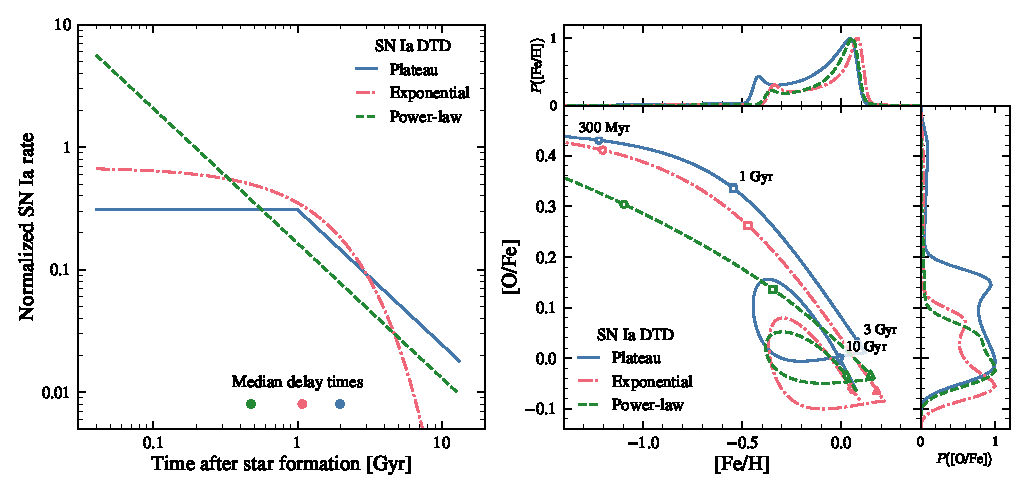
\includegraphics{figures/delay_time_distribution.pdf}
    \caption{Caption.}
    \label{fig:dtd}
\end{figure*}

We adopt the wide plateau DTD of \citet{dubay_galactic_2024} as our fiducial DTD.

\begin{equation}
    \label{eq:plateau-dtd}
    f_{\rm Ia}^{\rm plat}(t) =
    \begin{cases}
        1, & t < 1\,{\rm Gyr} \\
        (t/1\,{\rm Gyr})^{-1.1}, & t \ge 1\,{\rm Gyr}.
    \end{cases}
\end{equation}

\subsection{The Two-Infall Star Formation History}
\label{sec:sfh}

\todo{Copied from last paper.} First proposed by \citet{chiappini_chemical_1997}, this model parameterizes the infall rate as two successive, exponentially declining bursts to explain the origin of the high- and low-$\alpha$ disk populations:
\begin{equation}
    \label{eq:twoinfall-ifr}
    f_{\rm TI}(t|R_{\rm gal}) = N_1(R_{\rm gal}) e^{-t/\tau_1} + N_2(R_{\rm gal}) e^{-(t-t_{\rm on})/\tau_2},
\end{equation}
% In this model, the first infall produces the thick disk and the second infall produces the thin disk. 
where $\tau_1=1$ Gyr and $\tau_2=4$ Gyr are the exponential timescales of the first and second infall, respectively, and $t_{\rm on}=4$ Gyr is the onset time of the second infall \citep[based on typical values in, e.g.,][]{chiappini_chemical_1997,spitoni_galactic_2020,spitoni_apogee_2021}. $N_1$ and $N_2$ are the normalizations of the first and second infall, respectively, and their ratio $N_2/N_1$ is calculated so that the thick-to-thin-disk surface density ratio $f_\Sigma(R)=\Sigma_2(R)/\Sigma_1(R)$ is given by
\begin{equation}
    f_\Sigma(R) = f_\Sigma(0) e^{R(1/R_2 - 1/R_1)}.
\end{equation}
Following \citet{bland-hawthorn_galaxy_2016}, we adopt values for the thick disk scale radius $R_1=2.0$ kpc, thin disk scale radius $R_2=2.5$ kpc, and $f_\Sigma(0)=0.27$.
We note that most previous studies which use the two-infall model \citep[e.g.][]{chiappini_chemical_1997,matteucci_new_2006,matteucci_effect_2009,spitoni_galactic_2019} do not consider gas outflows and instead adjust the nucleosynthetic yields to reproduce the solar abundance. We adopt radially-dependent outflows as in \citetalias{johnson_stellar_2021} (see their Section 2.4 for details) for all our SFHs, including two-infall. We discuss the implications of this difference in Section \ref{sec:two-infall-discussion}.

The star formation law follows a single power-law prescription: $\dot\Sigma_\star\propto\Sigma_g^N$, with $N=1.5$ following \citet{kennicutt_global_1998}. Previous work with this GCE model \citep[e.g.,][]{johnson_stellar_2021,dubay_galactic_2024} assumed a three-component power-law, but we adopt a simpler prescription to allow for a more direct comparison with previous two-infall studies \citep[e.g.,][]{spitoni_remind_2024}. In detail, we calculate the star formation efficiency (SFE) timescale $\tau_\star\equiv\Sigma_g/\dot\Sigma_\star$ according to the following:
\begin{equation}
    \label{eq:sf-law}
    \tau_\star = 
    \begin{cases}
        \epsilon(t) \tau_{\rm mol}(t),   & \Sigma_g \ge \Sigma_{g,0} \\
        \epsilon(t) \tau_{\rm mol}(t) \Big(\frac{\Sigma_g}{\Sigma_{g,0}}\Big)^{-1/2}, & \Sigma_g < \Sigma_{g,0}
    \end{cases}
\end{equation}
where $\Sigma_{g,0} = 10^8\,{\rm M}_\odot\,{\rm kpc}^{-2}$ and $\tau_{\rm mol}(t)=\tau_{\rm mol,0}(t/t_0)^\gamma$ with $\gamma=1/2$ and $\tau_{\rm mol,0}=2$ Gyr. Previous two-infall studies \citep[e.g.,][]{nissen_high-precision_2020} have adopted a higher SFE during the first infall epoch than during the second, which we emulate through the pre-factor $\epsilon$:
\begin{equation}
    \label{eq:sfe-prefactor}
    \epsilon(t) = 
    \begin{cases}
        0.5, & t < t_{\rm on} \\
        1.0, & t \ge t_{\rm on}.
    \end{cases}
\end{equation}
\todo{Talk about the implications of this prefactor or reference a future section which discusses this.}

\subsection{Observational Sample}
\label{sec:observational-sample}

\begin{table*}
    \centering
    \caption{Sample selection parameters and median uncertainties from APOGEE DR17 (see Section \ref{sec:observational-sample}).}
    \label{tab:sample}
    \begin{tabular}{lll}
        \hline\hline
        \multicolumn{1}{c}{Parameter} & \multicolumn{1}{c}{Range or Value} & \multicolumn{1}{c}{Notes} \\
        \hline
        $\log g$            & $1.0 < \log g < 3.8$          & Select giants only \\
        $T_{\rm eff}$       & $3500 < T_{\rm eff} < 5500$ K & Reliable temperature range \\
        $S/N$               & $S/N > 80$                    & Required for accurate stellar parameters \\
        ASPCAPFLAG Bits     & $\notin$ 23                   & Remove stars flagged as bad \\
        EXTRATARG Bits      & $\notin$ 0, 1, 2, 3, or 4     & Select main red star sample only \\
        Age                 & $\sigma_{\rm Age} < 40\%$     & Age uncertainty from \citetalias{leung_variational_2023} \\
        \hline
        $\sigma({\rm [Fe/H]})$ & $9.2\times10^{-3}$ & Median uncertainty in [Fe/H] \\
        $\sigma({\rm [O/Fe]})$ & $1.8\times10^{-2}$ & Median uncertainty in [O/Fe] \\
        $\sigma($log(Age/Gyr)) & $0.10$ & Median age uncertainty \citepalias{leung_variational_2023} \\
        \hline
    \end{tabular}
\end{table*}

\todo{Copied from last paper.}
We compare our model results to abundance measurements from the final data release \citep[DR17;][]{abdurrouf_seventeenth_2022} of the Apache Point Observatory Galactic Evolution Experiment \citep[APOGEE;][]{majewski_apache_2017}. APOGEE used infrared spectrographs \citep{wilson_apache_2019} mounted on two telescopes: the 2.5-meter Sloan Foundation Telescope \citep{gunn_25_2006} at Apache Point Observatory in the Northern Hemisphere, and the Ir{\'e}n{\'e}e DuPont Telescope \citep{bowen_optical_1973} at Las Campanas Observatory in the Southern Hemisphere. After the spectra were passed through the data reduction pipeline \citep{nidever_data_2015}, the APOGEE Stellar Parameter and Chemical Abundance Pipeline \citep[ASPCAP;][]{holtzman_abundances_2015,garcia_perez_aspcap_2016} extracted chemical abundances using the model grids and interpolation method described by \citet{jonsson_apogee_2020}.

We restrict our sample to red giant branch and red clump stars with high-quality spectra. Table \ref{tab:sample} lists our selection criteria, which largely follow from \citet{Hayden2015-ChemicalCartography}. This produces a final sample of \input{output/sample_size.txt}stars with [O/Fe] and [Fe/H] abundance measurements. APOGEE stars are matched with their Bailer-Jones photo-geometric distance estimate from \textit{Gaia} Early Data Release 3 \citep{gaia_collaboration_gaia_2016,gaia_collaboration_gaia_2021}, which we use to calculate galactocentric radius $R_{\rm gal}$ and midplane distance $z$.

We use estimated ages from \citet[][hereafter \citetalias{leung_variational_2023}]{leung_variational_2023}, who use a variational encoder-decoder network which is trained on asteroseismic data to retrieve age estimates for APOGEE giants without contamination from age-abundance correlations. Importantly, the \citetalias{leung_variational_2023} ages do not plateau beyond $\sim10$ Gyr as they do in astroNN \citep{Mackereth2019-astroNN-Ages}. We use an age uncertainty cut of 40\% per the recommendations of \citetalias{leung_variational_2023}, which produces a total sample of \input{output/age_sample_size.txt}APOGEE stars with age estimates. We note that we use the full sample of \input{output/sample_size.txt}APOGEE stars unless we explicitly compare to age estimates. Table \ref{tab:sample} also presents the median uncertainties in the data for [Fe/H], [O/Fe], and age.

\section{Exploring the Parameter Space in One-Zone Models}
\label{sec:onezone-results}

\begin{figure}
    \centering
    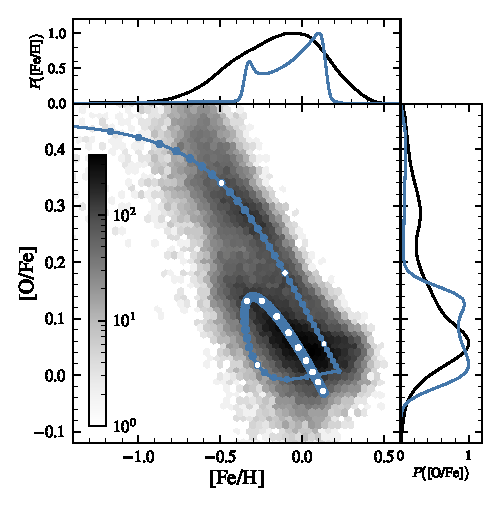
\includegraphics{figures/onezone_sfr.pdf}
    \caption{Caption.}
    \label{fig:onezone-sfr}
\end{figure}

\begin{figure*}
    \centering
    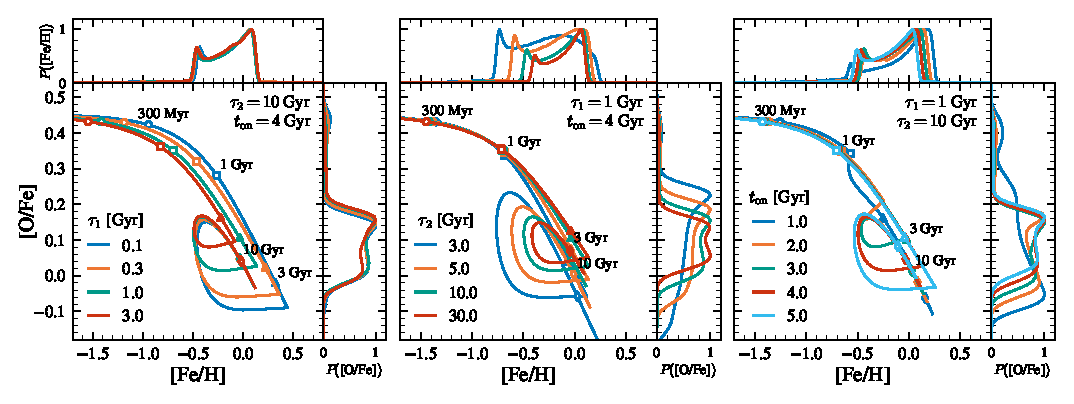
\includegraphics{figures/onezone_params.pdf}
    \caption{Caption.}
    \label{fig:onezone-params}
\end{figure*}

Figure \ref{fig:onezone-dtd} illustrates the effect of the SN Ia DTD on the abundance predictions by the two-infall model. The fiducial plateau DTD produces the strongest high-$\alpha$ peak as well as the greatest separation between the two low-$\alpha$ peaks. The exponential DTD produces the most stars near Solar [O/Fe], but the low-$\alpha$ sequence is still distinctly bimodal. Finally, the power-law DTD shrinks the low-$\alpha$ loop such that there is only one low-$\alpha$ peak; however, this DTD produces high-$\alpha$ stars at metallicities much lower than observed, as discussed in \citet{dubay_galactic_2024}.

\begin{figure*}
    \centering
    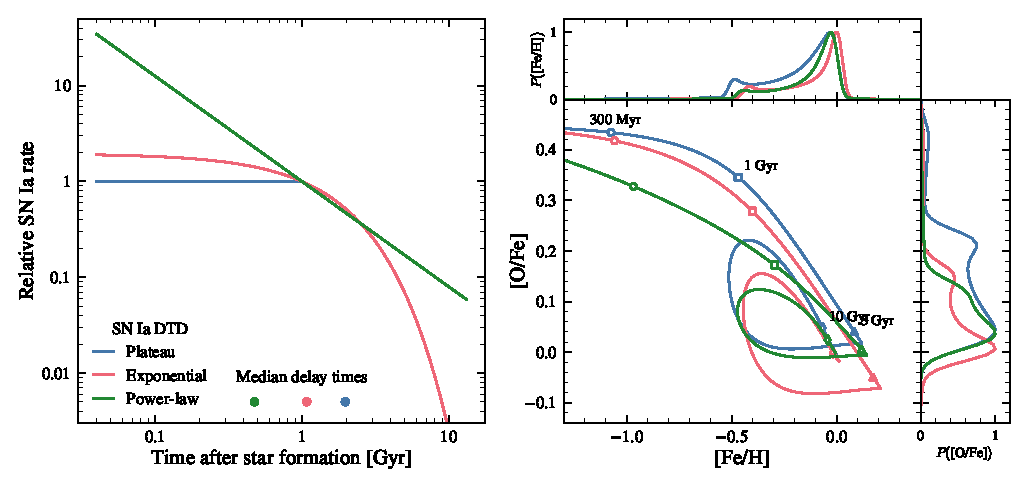
\includegraphics{figures/onezone_dtd.pdf}
    \caption{The model parameters are fixed at $\tau_1=1$ Gyr, $\tau_2=15$ Gyr, and $\tau_{\rm on}=3.2$ Gyr.}
    \label{fig:onezone-dtd}
\end{figure*}

\begin{figure}
    \centering
    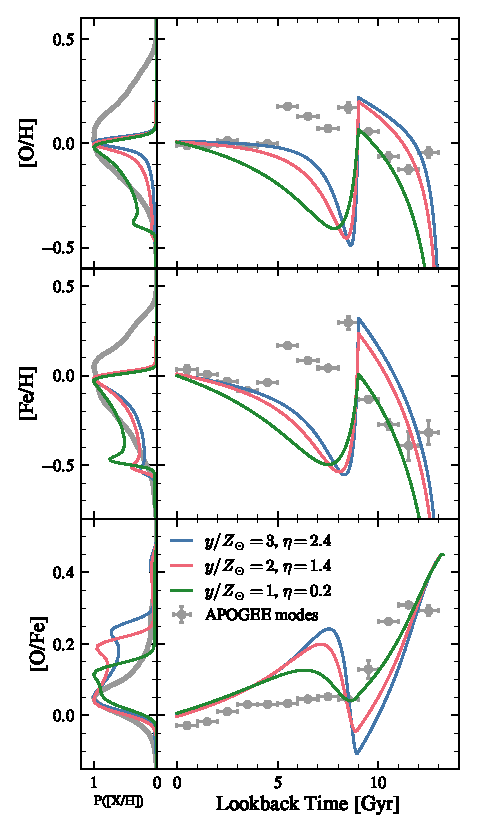
\includegraphics{figures/yield_outflow.pdf}
    \caption{Caption.}
    \label{fig:onezone-dtd}
\end{figure}

\section{Multi-Zone Models}
\label{sec:multizone-results}

\section{Discussion}
\label{sec:discussion}

\begin{figure}
    \centering
    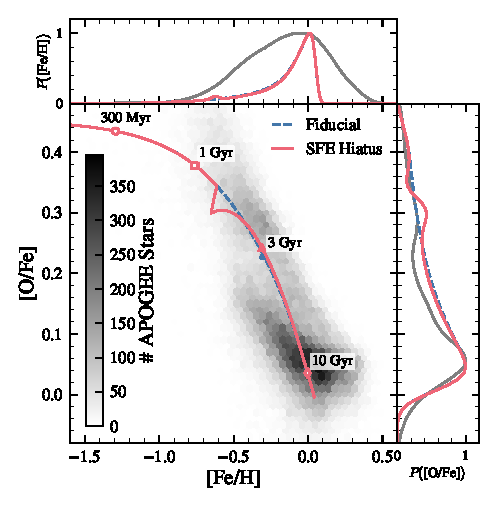
\includegraphics{figures/onezone_sfe_hiatus.pdf}
    \caption{Caption.}
    \label{fig:onezone-sfe-hiatus}
\end{figure}

\section{Conclusions}
\label{sec:conclusions}

\section*{Acknowledgements}

\todo{Personal acknowledgements.}

LOD and JAJ acknowledge support from National Science Foundation grant no.\ AST-2307621. JAJ and JWJ acknowledge support from National Science Foundation grant no.\ AST-1909841.
LOD acknowledges financial support from an Ohio State University Fellowship.
JWJ acknowledges financial support from an Ohio State University Presidential Fellowship and a Carnegie Theoretical Astrophysics Center postdoctoral fellowship. \todo{Update grants and fellowships.}

Funding for the Sloan Digital Sky 
Survey IV has been provided by the 
Alfred P.\ Sloan Foundation, the U.S.\ 
Department of Energy Office of 
Science, and the Participating 
Institutions. 

SDSS-IV acknowledges support and 
resources from the Center for High 
Performance Computing  at the 
University of Utah. The SDSS 
website is \url{www.sdss4.org}.

SDSS-IV is managed by the 
Astrophysical Research Consortium 
for the Participating Institutions 
of the SDSS Collaboration including 
the Brazilian Participation Group, 
the Carnegie Institution for Science, 
Carnegie Mellon University, Center for 
Astrophysics | Harvard \& 
Smithsonian, the Chilean Participation 
Group, the French Participation Group, 
Instituto de Astrof\'isica de 
Canarias, The Johns Hopkins 
University, Kavli Institute for the 
Physics and Mathematics of the 
Universe (IPMU) / University of 
Tokyo, the Korean Participation Group, 
Lawrence Berkeley National Laboratory, 
Leibniz Institut f\"ur Astrophysik 
Potsdam (AIP),  Max-Planck-Institut 
f\"ur Astronomie (MPIA Heidelberg), 
Max-Planck-Institut f\"ur 
Astrophysik (MPA Garching), 
Max-Planck-Institut f\"ur 
Extraterrestrische Physik (MPE), 
National Astronomical Observatories of 
China, New Mexico State University, 
New York University, University of 
Notre Dame, Observat\'ario 
Nacional / MCTI, The Ohio State 
University, Pennsylvania State 
University, Shanghai 
Astronomical Observatory, United 
Kingdom Participation Group, 
Universidad Nacional Aut\'onoma 
de M\'exico, University of Arizona, 
University of Colorado Boulder, 
University of Oxford, University of 
Portsmouth, University of Utah, 
University of Virginia, University 
of Washington, University of 
Wisconsin, Vanderbilt University, 
and Yale University.

This work has made use of data from the European Space Agency (ESA) mission
{\it Gaia} (\url{https://www.cosmos.esa.int/gaia}), processed by the {\it Gaia}
Data Processing and Analysis Consortium (DPAC,
\url{https://www.cosmos.esa.int/web/gaia/dpac/consortium}). Funding for the DPAC
has been provided by national institutions, in particular the institutions
participating in the {\it Gaia} Multilateral Agreement.

% From the Center for Belonging and Social Change, https://cbsc.osu.edu/about-us/land-acknowledgement
We would like to acknowledge the land that The Ohio State University occupies is the ancestral and contemporary territory of the Shawnee, Potawatomi, Delaware, Miami, Peoria, Seneca, Wyandotte, Ojibwe and many other Indigenous peoples. Specifically, the university resides on land ceded in the 1795 Treaty of Greeneville and the forced removal of tribes through the Indian Removal Act of 1830. As a land grant institution, we want to honor the resiliency of these tribal nations and recognize the historical contexts that has and continues to affect the Indigenous peoples of this land.

\software{\vice \citep{johnson_impact_2020}, Astropy \citep{astropy_collaboration_astropy_2013,astropy_collaboration_astropy_2018,astropy_collaboration_astropy_2022}, scikit-learn \citep{pedregosa_scikit-learn_2011}, SciPy \citep{virtanen_scipy_2020}, Matplotlib \citep{hunter_matplotlib_2007}}

\appendix

\section{Reproducibility}
\label{app:reproducibility}

\todo{Blah.}

\bibliography{references}

\end{document}
